\documentclass[10pt,a4paper]{article}

\usepackage{titlesec}
\usepackage[round]{natbib}
\usepackage{authblk}
\usepackage{fullpage}
\usepackage[space]{grffile}
\usepackage{graphicx}
\usepackage{textcomp}
\usepackage{deluxetable}
\usepackage{longtable}
\usepackage[utf8]{inputenc}
\usepackage[ngerman,english]{babel}
\usepackage{float}
\usepackage[margin=1in]{geometry}
\usepackage{parskip}
\usepackage{fixltx2e}


%\usepackage{setspace}
%\usepackage[section]{placeins}
%\usepackage{xcolor}
%\usepackage{breakcites}
%\usepackage{lineno}
%\usepackage{hyphenat}
%\usepackage{latexsym}
%\usepackage{tabulary}
%\usepackage{booktabs,array,multirow}
%\usepackage{amsfonts,amsmath,amssymb}


\renewcommand{\familydefault}{\sfdefault}


%\def\preprint{}


\PassOptionsToPackage{hyphens}{url}
\usepackage[colorlinks = true,
linkcolor = blue,
urlcolor = blue,
citecolor = blue,
anchorcolor = blue]{hyperref}
\usepackage{etoolbox}
\makeatletter
%\patchcmd\@combinedblfloats{\box\@outputbox}{\unvbox\@outputbox}{}{%
% \errmessage{\noexpand\@combinedblfloats could not be patched}%
%}%
\makeatother



\renewenvironment{abstract}
 {{\bfseries\noindent{\abstractname}\par\nobreak}\footnotesize}
 {\bigskip}


% You can conditionalize code for latexml or normal latex using this.
\newif\iflatexml\latexmlfalse
\providecommand{\tightlist}{\setlength{\itemsep}{0pt}\setlength{\parskip}{0pt}}%

\AtBeginDocument{\DeclareGraphicsExtensions{.pdf,.PDF,.eps,.EPS,.png,.PNG,.tif,.TIF,.jpg,.JPG,.jpeg,.JPEG}}



% Edit this header.tex file to include frontmatter definitions and global macros
\newcommand{\beginappendix}{%
	\setcounter{table}{0}
	\renewcommand{\thetable}{A\arabic{table}}%
	\setcounter{figure}{0}
	\renewcommand{\thefigure}{A\arabic{figure}}%
}

% Add here any LaTeX packages you would like to load in all document blocks


% Add here any LaTeX macros you would like to load in all document blocks
% \def\example{This is an example macro.}

% -----

\iflatexml
% Add here any LaTeXML-specific commands

% -----

\else
% Add here any export style-specific LaTeX commands. These will only be loaded upon document export. 
% \paperfield{Subject domain of my document}
% \keywords{keyword1, keyword2}
% \corraddress{Author One PhD, Department, Institution, City, State or Province, Postal Code, Country}
% \fundinginfo{Funder One, Funder One Department, Grant/Award Number: 123456.}
\fi


\begin{document}

\title{Why do we have so many different hydrological models? A review based on the case of Switzerland}


\author[1]{Pascal Horton*}
\author[1]{Bettina Schaefli}
\author[1]{Martina Kauzlaric}
\affil[1]{Institute of Geography \& Oeschger Centre for Climate Change Research, University of Bern, Bern, Switzerland (pascal.horton@giub.unibe.ch)}


 \date{}


\ifdefined\preprint
\setcounter{page}{0}
\hrulefill

This manuscript has been submitted for publication in \textbf{WIREs Water}. Please note that it has not been peer reviewed and has not yet been accepted for publication. Subsequent versions of this manuscript may have different content. If accepted, the final version of this manuscript will be available via the ‘Peer-reviewed Publication DOI’ link on the right-hand side of this webpage. Please feel free to contact any of the authors; we welcome feedback

\hrulefill
\newpage
\fi

\begingroup
%\let\center\flushleft
%\let\endcenter\endflushleft
\maketitle
\endgroup




\begin{abstract}
Hydrology plays a central role in applied as well as fundamental environmental sciences, but it is well known to suffer from an overwhelming diversity of models, in particular to simulate streamflow. Based on Switzerland's example, we discuss here in detail how such diversity did arise even at the scale of such a small country. The case study's relevance stems from the fact that Switzerland shows a relatively high density of academic and research institutes active in the field of hydrology, which led to an evolution of hydrological models that stands exemplarily for the diversification that arose at a larger scale. Our analysis summarizes the main driving forces behind this evolution, discusses drawbacks and advantages of model diversity and depicts possible future evolutions. Although convenience seems to be the main driver so far, we see potential change in the future with the advent of facilitated collaboration through open sourcing and code sharing platforms. We anticipate that this review, in particular, helps researchers from other fields to understand better why hydrologists have so many different models.
\end{abstract}%


\section{Introduction}
\label{sec:intro}

Hydrological models are essential tools for hydrologists, be it for operational flood forecasting, water resource management or the assessment of land use and climate change impacts. Since the advent of hydrological modelling, the number of models keeps increasing at a fast pace. It has become common to talk about the ``plethora of hydrological models'' (index term found more than 13'400 times in a Google search on 11 Jan 2021). Single models are branching out into numerous variants, such as the Hydrologiska Byråns Vattenbalansavdelning model (HBV; \citealp{Bergstrom1976a, Bergstrom1992, Bergstrom1995, Lindstrm1997})  that exists in multiple versions nowadays. Some authors support the idea that there are too many hydrological models, which might lead to a waste of time and effort, and that the hydrological community should gather on a Community Hydrological Model \citep{Weiler2015}.

While any newcomer to hydrological modelling will easily find some guidance on navigating the sheer diversity of hydrological models, understanding the concepts and limitations \citep{Beven2013, Solomatine2011, Kauffeldt2016}, the question of how this diversity has emerged receives much less attention. Existing historical analyses of model diversity \citep{Peel2020} generally focus on the technical evolution of model types. According to our personal experience, much of the knowledge about why many similar models have emerged is transferred informally.

One of the key drivers for the pronounced model diversity in hydrology is certainly the wide range of model applications \citep{Weiler2015} that all require \textit{appropriate modelling}; this concept can be defined following \citet{Rosbjerg2005} as ``the development or selection of a model with a degree of sophistication that reflects the actual needs for modelling results''. Two well-accepted characteristics that models should exhibit are parsimony and adequacy to the problem at hand, i.e. a model should not be more complex than necessary and should be fit-for-purpose \citep{Beven2013}. Indeed, a model developed for droughts cannot be blindly applied to the assessment of floods. Also, catchments with different properties or climatology may require different model structures \citep{Kavetski2011, vanEsse2013}. In other words, the hydrological model diversification is strongly driven by the modelling context and by what is now often called \textit{uniqueness of place} \citep{Beven2000}.

However, the hydrologic literature also offers other explanations, ranging from legacy reasons for model selection \citep{Addor2019}, to a lack of agreement on concepts for process representations and to the simple wish to try to do better with yet another model parameterization \citep{Weiler2015}.

We attempt here an analysis of what might explain the emergence of multiple hydrological models at a rather small scale, the scale of Switzerland, a country small enough to do an exhaustive analysis, but diverse enough to shed light on some of the most dominant drivers of model diversity. Despite Switzerland's small area (41285 km\textsuperscript{2}), numerous models are being developed and applied in the same contexts and often even for the same purpose and the same catchment. 

Thus, this work aims to disentangle the motivations and reasons behind the choices that led to the current co-existence of a wide range of models. We focus this analysis on hydrological models (see Box 1) that simulate hydrological processes, including surface and subsurface flow, and the resulting streamflow at the catchment scale. Some of these models are classical rainfall-runoff models (Box 1), while others have more specific purposes. We exclude here models that simulate the water balance without providing streamflow at the catchment outlet. We first briefly present the different models used in Switzerland (Section \ref{sec:models}), and attempt a classification according to types of application and research fields (Section \ref{sec:application}), before presenting a synthesis of our findings on drivers of model diversity (Section \ref{sec:motivations}) and conclusions (Section \ref{sec:conclusion}).


\begin{quote}
\subsection*{Box 1: What do we mean by hydrological model ?}
\label{box:1}

A hydrological model is an input-output model that simulates the evolution of water storage, of water fluxes and potentially of associated chemical and physical properties at the Earth's surface and subsurface, based on the water balance equation. The term ``rainfall-runoff model'' is often used for hydrologic models that simulate streamflow at a catchment outlet based on input time series of rainfall. The term ``rainfall-runoff'' stems from the early times when such models simulated how much water of a rainfall event ran off to the stream (rather than being stored in the catchment), i.e. ``runoff'' designated the part of rainfall that appears as streamflow \citep{WMO1992}. Nowadays, rainfall-runoff models are continuous simulation tools that simulate all components of streamflow (including baseflow), and the term ``runoff'' now designates the lateral (as opposed to vertical) movement of water (at the surface or in the subsurface) towards a river \citep{WMO2012}. Modern rainfall-runoff models further transform simulated hillslope-scale runoff to catchment-scale streamflow; some of them include instream routing. Such models can be generalized to precipitation-runoff models in the presence of snowfall. The term ``water balance model'' is sometimes used as synonym for rainfall-runoff models \citep{Boughton2004} . The correcter term ``rainfall-streamflow'' model appeared rather early \citep{Young1991} but is to date (12 Jan 2021) only used in 17 WebOfScience publications. Streamflow is in many papers called interchangeably ``discharge'' and sometimes even ``runoff'', which is a legacy effect.  \end{quote}


\section{Hydrological models developed and used in Switzerland}
\label{sec:models}

\subsection{Preliminary remark}
\label{sec:models:remark}

The information sources considered in this analysis are as far as possible peer-reviewed articles with applications to hydrology. The articles were retrieved based on searches by authors (hydrologists in Switzerland) and keywords. While we tried to search all applications as exhaustively as possible, biases in the search and citing network effects are possible if not likely. Where necessary, conference proceedings, PhD theses, research and government reports are also included. A few models are exclusively used or developed in engineering companies, and these are not included here. Furthermore, our analysis focuses on catchment-scale modelling and excludes studies that focus on hydrogeological modelling \citep{Carlier2019} and those with a focus on urban hydrology \citep{Peleg2017} or urban hydrogeology \citep{Schirmer2013}. All articles are not directly referenced in this paper, but a complete table is available in the supplementary material.


\subsection{History of hydrological modelling in Switzerland}
\label{sec:models:history}

The early times of hydrological modelling in Switzerland can be situated in the years 1970 to 1990, when model diversity naturally emerged in response to modelling needs. From a hydrological processes perspective, a strong focus was on the simulation of snowmelt runoff \citep{Braun1986} as well as on understanding the role of forests in the water cycle \citep{Keller1991, Forster1989}. Along with modelling studies in experimental catchments \citep{Iorgulescu1994}, first model-based climate change \citep{Bultot1992a} and land-use change \citep{Jordan1990a} impact studies appeared. Quantitative real-time forecasts for water resources management \citep{Lugiez1969} and hydropower production \citep{Jensenlang1973} started being based on hydrologic models rather than statistical approaches.

It is worth noting that \citet{Naef1977} presented already a first model intercomparison study, comparing complex and simple models. In fact, model diversity already started interpellating the research community in the late 1970ties and \citet{Naef1981} notably asked: ``But, given that the results are good, why do new models continue to be published?'' 

From a historical analysis (see Supplementary Information), one interesting aspect can be retained: already in the early times of model development, part of the model diversity resulted from the work of geoscientists and engineers not directly specialized in catchment hydrology \citep{Abednego1990, Baumgartner1986a, Hager1984, Sautier1980}, which partly explains the parallel emergence of similar models. 

Additional details on the emergence of hydrological modelling in Switzerland are given in the Supporting Information. For a more general dive into the history of modelling, the reader is referred to the work of Keith Beven \citep{Beven2020,Beven2020a}.


\subsection{Model overview}
\label{sec:models:overview}

There are several hydrological models that have been developed in Switzerland (Table \ref{tab:modelslist}), ranging from rainfall-runoff models (PREVAH, GSM-SOCONT, RS, SEHR-ECHO, WaSiM), to snow-based models (ALPINE3D), glacier-hydrology models (GERM) and water temperature models (StreamFlow). Some models (Table \ref{tab:modelslist}) have their roots outside Switzerland but are now actively being developed in Switzerland (HBV-light, TOPKAPI-ETH, SUPERFLEX) or were applied to Swiss case studies (CemaNeige-GR6J, LARSIM, VIC, SWAT, mHM). 

All these models are briefly described in Appendix 1. Switzerland being an Alpine country, most of these models include a representation of snow accumulation and melt, some also include glacier-related processes.


\hspace{-4cm}\begin{deluxetable}{l l l c}[htb]
	\vskip4mm
	\centering
	\tabletypesize{\footnotesize}
	\tablecolumns{4} 
	\tablecaption{List of models (alphabetical order) applied in Switzerland; the fourth column indicates whether the model was originally developed (D) or further evolved (E) by teams active at Swiss universities or research institutes, or whether it is only applied to Swiss case studies, either by teams active in Switzerland (A-CH) or by teams active abroad (A). References are in the main text and Appendix 1. \label{tab:modelslist}}
	\tablewidth{0pt}
	\tablehead{
		\colhead{Model name} & \colhead{Full name} & \colhead{Spatial structure} & \colhead{Type of use}}
	\startdata 
	ALPINE3D & ALPINE3D & distributed & D  \\
	CemaNeige-GR6J & CemaNeige - Genie Rural \`{a} 6 param\`{e}tres Journalier & lumped & A-CH \\
	DECIPHeR & Dynamic fluxEs and ConnectIvity for Predictions of HydRology & HRU-based & E \\
	GERM & Glacier Evolution Runoff Mode & distributed & D \\
	GSM-SOCONT  & Glacier and SnowMelt {SOil CONTribution model} & semi-distributed & D  \\
	HBV & Hydrologiska Byråns Vattenbalansavdelning & semi-distributed & A\\
	HBV-light & Hydrologiska Byråns Vattenbalansavdelning - light & semi-distributed &  E  \\
	HYPE  & HYdrological Predictions for the Environment & semi-distributed &  A  \\
	LISFLOOD & LISFLOOD & distributed &  A \\
	LARSIM & Large Area Runoff Simulation Model & semi-distributed &  A \\
	mHM & meso-scale hydrological model & distributed &  A \\
	PREVAH & Precipitation-Runoff-Evapotranspiration HRU Model & HRU-based \& distributed &  D  \\
	RS & Routing System & semi-distributed &  D  \\
	SEHR-ECHO  & Spatially Explicit Hydro. Response model for ecohydro. applic. & semi-distributed &  D  \\
	StreamFlow & StreamFlow & distributed &  D  \\
	SUPERFLEX & SUPERFLEX & (not fixed) &  E  \\
	SWAT  & Soil Water and Assessment Tool & semi-distributed &  A-CH,A \\
	TOPKAPI-ETH & TOPographic Kinematic APproximation and Integration - ETH & distributed &  E  \\
	VIC & Variable Infiltration Capacity model & distributed &  A \\
	WaSiM(-ETH) & Water Flow and Balance Simulation Model (- ETH) & distributed &  D  \\
	wflow & wflow & distributed &  A  \\
	\enddata
\end{deluxetable}



\section{Diversity drivers from applications}
\label{sec:application}

The alpine environment is a complex system with specific processes that play a dominant role in the hydrological cycle. For that reason, the choice and the development of models are driven by the dominant natural processes as well as the characteristics of such environment. For example, PREVAH is presented by \citet{Anghileri2019} as being “specifically designed to capture hydrological processes that are important for catchments in complex terrain”, and multiple similar statements can be found in the literature \citep{Verbunt2007, Zappa2007a, Koplin2010,  Brunner2019e}. This is also true for other models such as WaSiM \citep{Jasper2002, Jasper2003, Thornton2021} or HBV-light \citep{SikorskaSenoner2020}. 

The great variability of local conditions in alpine environments, such as slope, orientation and elevation, is a driver for an increased spatial resolution in hydrological models compared to regions with more gentle topography \citep{Gurtz2003}. Indeed, most models used and developed in Switzerland are semi-distributed of fully distributed. Very few applications rely on lumped models \citep[for example,][]{Keller2019a}. Topography has a strong impact on the meteorological forcing, whether for precipitation, temperature, or solar radiation. For this reason, some semi-distributed models such as GSM-SOCONT and HBV-light have a discretization in elevation bands.

While natural processes and characteristics of the landscape have an impact on model selection and development, the context of the model application can also play a role, for example in terms of computing efficiency for climate change impact studies on long periods, or data assimilation for operational forecasting. We attempt here a clustering of modelling studies according to either the representation of key processes in the model (Sect. \ref{sec:application:processes}) or the influence of the application context (Sect. \ref{sec:application:context}) in various Swiss catchments (Fig. \ref{fig:map}).


\begin{figure}[htb]
	\begin{center}
		\includegraphics[width=0.95\columnwidth]{figures/map}
		\caption{{Map of Switzerland with its major drainage divides (green), the extent of the ``hydrological Switzerland'' (orange) and some catchments (brown) that are referenced in the text (Data: Federal Office of Topography swisstopo and Hydrological Atlas of Switzerland). \label{fig:map}
		}}
	\end{center}
\end{figure}


\subsection{Process-driven influences}
\label{sec:application:processes}


\subsubsection{Cryosphere-related processes}
\label{sec:application:cryosphere}

Snow and glaciers are key components of the alpine environment as they play a major role on hydrological regimes through a temporal redistribution of water. These processes thus need to be accurately represented in the models, which can be achieved with different levels of complexity. 

For example, most hydrological models used in Switzerland rely on a simple temperature-index based snow routine \citep[see for example][]{Jenicek2018}. On the other end, ALPINE3D, which is built on the physically-based SNOWPACK model (\citealt{Bartelt2002, Lehning2002a, Lehning2002b}), has certainly the most complex representation of snow processes among Swiss models. It allows analyses that require a fully distributed and physically-based approach to snow modelling, such as the influence of solar radiation patterns \citep{Comola2015a} or snow distribution and water transport within the snowpack \citep{Brauchli2017} on the catchment-scale hydrologic response, or the influence of snow processes on the soil moisture and streamflow \citep{Wever2017}. However, detailed comparisons between simple snow routines and ALPINE3D have not been conclusive so far with respect to climate change applications \citep{Kobierska2011, Shakoor2018}.

In the context of climate change impact on snow processes, ALPINE3D was used by \citet{Bavay2009} to assess the future snow cover and the related discharge in two alpine catchments with different size. The emphasis of ALPINE3D on snow processes drove the choice of the model. Its physically-based approach to snow processes implies heavier computation, which can be a limitation for climate change impact studies using ensemble approaches or simulations on long periods. Other uses of ALPINE3D in climate impact studies rely so far on a limited number of members \citep[climate scenarios or climate model chains;][]{Bavay2013, Marty2017}. Another complex snow routine has been implemented in WaSiM and was shown to provide reliable results for distributed snow simulations \citep{Thornton2021}. 

Most models developed in Switzerland have a glacier module, even the bucket-type models, and are used to quantify the contribution of glaciers to the hydrological response of a catchment \citep[see for example][]{Verbunt2003, Zappa2007a, Uhlmann2013a}. Applications to glacierized catchments can also drive further improvement of snow and glacier melt representation in the model \citep{Finger2011}. ALPINE3D was also used in this context by \citet{Hindshaw2011} to attribute the origin of systematic seasonal and diurnal variations in glacial stream water chemistry.

The impact of glacier retreat on hydrology is at the heart of many climate impact studies \citep{Horton2006, Schaefli2007b, Junghans2011, Addor2014, Finger2015, Etter2017}. This namely gave rise to the development of the GERM model \citep{Huss2016, Junghans2011, Farinotti2012, Finger2013}, which focuses on glacier processes, and a new glacier retreat parameterization scheme widely applied internationally \citep{Huss2010}.



\subsubsection{Hydraulic infrastructures and hydropower operations}
\label{sec:application:infrastructures}

Streamflow in the Swiss Alps can be heavily influenced by antropic infrastructures, such as water diversion and hydropower operations. Thus, specific modules need to be implemented in hydrological models to account for these aspects, which is the case of several models. For example, TOPKAPI-ETH was chosen by \citet{Fatichi2014} as it "is designed to account for hydraulic infrastructures such as reservoir and river diversions as well as for water withdrawals for irrigation and domestic/industrial water consumption". It was also used for studies targeting hydropower operations in a climate change context \citep{Fatichi2015b, Anghileri2018}. WaSiM has also a module for hydropower activities \citep{Verbunt2005}.

Hydraulic infrastructures and hydropower operations are at the core of RS MINERVE, which was designed primarily for that application. In consequence, it was also coupled with other hydrological models, such as PREVAH, to account for these influences \citep{Andres2016, Stucki2018}.
 

\subsubsection{Sediment production and transport}
\label{sec:application:sediments}

A special topic that deserves some focus is sediment transport modelling. The modelling of sediment sources, as well as transport capacity, requires models that yield reliable spatial patterns of hydrological processes, i.e. distributed models such as TOPKAPI-ETH, which has been modified to account for river bed erosion and deposition processes using a sub-grid modelling scheme \citep{Konz2011}. This modification allows the simulation of erosion and deposition patterns, sediment transport rates, and evolution of the channel slope. \citet{Battista2020a} later developed a new soil erosion and sediment transport module for TOPKAPI-ETH. They investigated the effects of precipitation and surface erodibility and their spatial variability on sediment fluxes. This new module was then used by \citet{Battista2020} to analyze the role of localized sediment sources, such as incised areas and landslides. They conclude that accounting for localized sediment sources improves sediment transport modelling and allows sediment sampling optimization and support of sediment provenance studies.

Sediment management, for example in the context of hydropower production \citep{RaymondPralong2015,Gabbud2016}, is constantly gaining importance in Alpine countries and will most likely drive the development of new modules to simulate the interplay of hydrological and geomorphological processes at the catchment scale. In Switzerland, climate change is expected to decrease the sediment yield in average due to reduced runoff in summer, and to shift the sediment transport regime to earlier months \citep[as found by ][using PREVAH]{RaymondPralong2015}.


\subsubsection{Ecohydrology and water quality}
\label{sec:application:ecohydrology}

Ecohydrology studies the feedbacks between ecosystems, in particular with vegetation and the water cycle \citep{Tague2020}. To date, catchment-scale studies with ecohydrological models accounting for feedback with vegetation are scarce in Switzerland. An early example is a work of \citet{Zierl2005}, who used the model RHESSys to study climate and land-use change impacts on alpine streamflow in Switzerland. Later, \citet{Fatichi2012, Fatichi2012a} developed an ecohydrological model, called Tethys-Chloris (T\&C), to simulate vegetation-hydrology interactions at large scales. It has been applied to catchments in Switzerland to study soil moisture spatiotemporal dynamics \citep{Fatichi2015a}, as well as to assess the vulnerability of Alpine ecosystems to climate change \citep{Mastrotheodoros2019}.

Another approach consists in coupling ecosystem models to distributed hydrological models, such as TOPKAPI-ETH in the analysis of the interactions between rivers, aquifers and ecosystems \citep{Foglia2009, Pappas2015}, or PREVAH in the assessment of the climate change impact on brown trouts \citep{Junker2015}. The impact of vegetation changes on streamflow can also be to some extent modelled as a change in land use, such as done in several analysis of forest change by \citet{Koplin2013} and \citet{Schattan2013} with PREVAH and by \citet{Alaoui2014} with WaSiM.

Water quality is also likely to become a growing concern, which might lead to an increase in studies on transport of chemicals \citep{queloz2015}, nutrients and pollutants, on C0\textsubscript{2} production or water temperature \citep{Michel2020}. Water quality and nutrient loads in the Thur catchment have been modeled by \citet{Abbaspour2007} using SWAT. The objective of the study was to test the performance of the model for such application. They concluded that "in watersheds similar to Thur – with good data quality and availability and relatively small model uncertainty – it is feasible to use SWAT". 


\subsubsection{Agricultural water use and impacts}
\label{sec:application:agriculture}

There are very few studies on agricultural water use, a topic that will likely gain importance in the future, but that might not further drive model diversification. For example, WaSiM has already been shown to be suitable to study the demand and supply of water for agriculture, including irrigation \citep{Fuhrer2012}. Besides, internationally widely used models might see more applications in Switzerland. One such example is SWAT, which - given its user-friendliness \citep{Abbaspour2007} - is likely to see more alpine applications despite not being specifically designed for alpine environments \citep{Rahman2014, Andrianaki2019}, but in exchange offers the option to study land management effects \citep{Zarrineh2018} or the joint effect of land use and climate change \citep{Rahman2015}. SWAT was also applied by \citet{Zarrineh2020} to an agricultural region in Western Switzerland to assess the impact of climate change on streamflow, erosion, and agriculture.


\subsection{Context-driven influences}
\label{sec:application:context}


\subsubsection{Analysis of model behaviour and uncertainty analysis}
\label{sec:application:uncertainty}

A large body of the hydrologic modelling literature focuses on a better understanding of model behaviour and in particular of model performance with respect to reproducing observed streamflow, e.g. as a function of model parameterizations, of spatio-temporal model resolution \citep{Brunner2019}, of precipitation input data \citep{Sikorska2016, Sikorska2017, MullerThomy2019}, or of parameter estimation techniques \citep{Foglia2009, Cullmann2011}. In the context of model diversity, this field of research has overall little impact because most modelling groups who work on such theoretical aspects often use their in-house models for proofs of concepts or to improve them (e.g. \citealt{Schaefli2007, Hingray2010}).

Model performance studies cover, for example, the integration of glacier mass balance data \citep{Finger2015, Schaefli2011}, snow data assimilation \citep{Griessinger2016}, accounting for streamflow observation uncertainty \citep{Westerberg2020}, the influence of spatial or temporal resolution of hydro-meteorological input \citep{GironsLopez2016, Felder2017, Sikorska2018}, integration of citizen science data \citep{Etter2020}, error correction in forecasting chains \citep{Bogner2018}, assessment of spatial pattern reproduction of soil moisture and evapotranspiration \citep{Rossler2010, Zappa2003} and of snow \citep{Zappa2008a}, and the comparison of various climate postprocessing methods \citep{Rossler2019}.

Overall, there are only few parameter regionalisation studies. A first example is the work of \citet{Viviroli2015}, where the benefit of a combination of parameter regionalisation and short-term runoff measurements for catchments without extensive data has been investigated. Another example is the work of \citet{Melsen2016}, who applied the internationally used VIC model to the Thur catchment to assess the impact of parameter transfer over different temporal and spatial resolutions.


\subsubsection{Characterization and quantification of floods and droughts}
\label{sec:application:floodsdroughts}

Infrastructure planning, water resources and natural risk management also heavily rely on probabilistic quantifications of extremes, i.e. an estimation of what could happen in terms of floods and droughts and their associated probabilities (called return periods in hydrology). Work in this field continues to be based on statistical analyses and extrapolation of observed streamflow time series \citep{Brunner2018, Asadi20108}, but hydrological models play an ever-increasing role to complement missing or insufficient streamflow data.

Any model-based flood estimation method is computationally intensive since long model simulation runs are required at an hourly time step \citep[see][about reducing computational requirements for extreme flood estimation by hydrological modelling]{SikorskaSenoner2020}. Accordingly, simple models such as PREVAH \citep{Viviroli2009, Viviroli2009c, Felder2017}, HBV-light \citep{Sikorska2017, Brunner2019a, SikorskaSenoner2020} and  RS \citep{Bieri2013, Zeimetz2017, Zeimetz2018} are often used for flood estimation; these models are all deemed to perform well enough for flood estimation in Swiss catchments by their respective authors and users. To bring diversity in the type of models used for flood modelling, the open-source DECIPHeR model is being futher developed and implemented for Swiss catchments (Kauzlaric, personal communication).

Other more complex distributed models, such as WaSiM, are also used for flood modelling, but more often on an event-based temporal scale, as for example in the case of a reconstruction of the 1816 Tambora eruption and its impact on floods in the upper Rhine basin \citep[see Fig. \ref{fig:map};][]{Rossler2018}. Such model can be highly relevant to study specific flood types that involve a good physical parameterization of small scale processes, such as rain-on-snow flood events, as in the study by \citet{Rossler2014}. Despite relatively long simulation time, WaSiM has also been used to model longer periods as in the assessment of climate change impacts on floods characteristics \citep{Keller2019a}. A physically-based model was also needed for the analysis of \citet{Paschalis2014} with TOPKAPI-ETH on the interplay of rainfall's temporal variability and the clustering of saturated areas in flood generation.

Work on droughts is much less abundant in Switzerland than work on floods, which is related to the fact that missing water was, in the past, not a hot topic in this country known as the water tower of Europe \citep{Milano2015}. What can be highlighted here is that the same models are in use to assess droughts and floods, potentially with specific recalibration, but without modifictaion of the model structure. This is motivated by the fact that existing models are deemed to reproduce well all dominant processes in the Swiss environment, as e.g. explicitly stated in the work of \citet{Zappa2007a} on quantifying the hydrological impact of the 2003 heatwave with a distributed version of PREVAH. It was also later on used for additional drought analyses \citep{Brunner2019e, Zappa2019}, where a spatial mismatch between water scarcity and storage availability has been highlighted for Switzerland \citep{Brunner2019e}. Similarly, HBV-light served in several drought studies, such as for the definition of a new drought index that accounts for snow \citep{Staudinger2014}, the predictability of low flows \citep{Staudinger2014a}, or the sensitivity of catchments to meteorological droughts \citep{Staudinger2015}. It was also used to assess low flow drivers in Alpine catchments \citep{Arnoux2020}. However, significant efforts to improve the model representation of groundwater and the corresponding baseflow during droughts remain to be done in Switzerland, which might lead to further model diversification.


\subsubsection{Climate change impact analysis}
\label{sec:application:climatechange}

Climate change impact studies emerged in Switzerland in the 1990s, including a large national research programme on climate change and natural hazards \citep{SNFS2021}. Since then, all model-based studies are mostly conducted with the models that established themselves in Switzerland, which have, however, not been specifically designed for climate change impact analysis; detailed assessments of how well these models can simulate future conditions are largely missing. Climate change impact analyses require, among others, a good representation of the processes that play a key role in the studies. The representation of these processes in the models is discussed in Sect. \ref{sec:application:processes}, both for present and future climate conditions. These studies also require models that are not too time consuming due to processing of long transient periods as well as due to increasing ensemble size of modelling chains.

WaSiM was chosen by \citet{Middelkoop2001} for a climate change impact study primarily due to its good interpolation of meteorological data for mountain environments, and by \citet{Jasper2004} to assess the effect of different regional climate scenarios in the Thur and the Ticino catchments (Fig. 1). WaSiM has also been applied to assess future soil water patterns \citep{Jasper2006, Rossler2012} and future summer evapotranspiration regimes \citep{Calanca2006}, applications where a more physically-based representation of vertical and horizontal flow processes -- involving the Richards equation -- is important. It was even applied for the entire Rhine basin at a 1~km\textsuperscript{2} resolution down to Rotterdam by \citet{Kleinn2005}.

TOPKAPI-ETH, the other frequently used physically-based distributed model has also been applied to several climate change impact studies, such as in the analysis of internal climate variability \citep{Fatichi2014}, or the assessment of future water resources \citep{Finger2012}. It was also selected by \citet{Fatichi2015}, who argues that “it represents a reasonable compromise between physically meaningful representation of hydrological processes and computational time for large-scale ($>$1000~km\textsuperscript{2}), long-term ($>$20~yr), high-resolution ($<$1~km\textsuperscript{2}) distributed simulations”.

The most widely used models to study climate change impact on streamflow are to date however the reservoir-based models PREVAH (\citealt{Koplin2012, Speich2015, Milano2015a, Brunner2019c} and others;  see Supplementary material) and HBV-light (\citealt{Etter2017, Hakala2020, Brunner2018a, Jenicek2018}  and others). In the western part of Switzerland, RS MINERVE and GSM-SOCONT have been used, especially for high elevation sites \citep{Horton2006, Uhlmann2013a, Uhlmann2013b, Terrier2015}. The justification of these models for climate change impact assessments is well summarized by \citet{Koplin2010} who, for PREVAH, states that the model ``has been developed especially to suit conditions in mountainous environments'' and that it ``has proved to be a reliable and flexible tool for various scopes of application and climate conditions ranging from drought analysis over water balance modelling to flood estimation and forecasting''. 

In this context, we would like to stress here that there are still relatively few examples of hydrologic model ensembles (using several hydrologic models) for climate change impact assessment \citep{Kobierska2011, Bosshard2013a, Addor2014}. The expectations in this regard might raise in the future, requiring the use of additional, and likely internationally widely applied, hydrological models.


\subsubsection{Operational forecasting}
\label{sec:application:forecasting}

The ever increasing need for reliable real-time streamflow forecasts leads to a continuous evolution of the underlying hydro-meteorological modelling systems. Real-time forecasting started with deterministic forecasts from a single meteorological forecast applied to a single hydrological model; today, users expect full stochastic ensemble forecasts at hourly time scales, updated every few hours and with several stochastic meteorological inputs applied to different hydrological models \citep{Jasper2016}. Coupled atmospheric--hydrologic ensemble prediction systems were proven to provide better forecasts than deterministic simulations \citep{Verbunt2007, Zappa2008, Jaun2008, Liechti2013}. These might also include data assimilation schemes \citep{JorgHess2015a} or the assessment of hydrologic uncertainty related to meteorological forcings, model parameters and initial conditions \citep{Jaun2009, Zappa2011a, Fundel2011}.

Such modern forecasting systems require hydrological models that provide forecasts at many locations in a stream network and that include the effect of hydraulic infrastructures (eg. of hydropower water intakes and accumulation lakes). Since the early times of flood forecasting in Switzerland, HBV and PREVAH were used in governmental offices \citep{Jasper2016} as well as in research institutes because of their relative simplicity and low computational costs \citep{Verbunt2006, Addor2011, Murphy2019, Antonetti2019}. Along with HBV, PREVAH and LARSIM, WaSiM is today part of the Swiss operational ensemble forecasting system \citep{Jasper2016}, which uses the FEWS platform (Flood Early Warning System; \citealp{Werner2013}) to provide forecasts for the cantonal authorities and the public \citep{FOEN2019}. A key advantage of the WaSiM model is the fact that it can explicitly account for lake regulations and hydropower operations (J. Schulla, personal communication, October 23, 2020). WaSiM has also been used for research studies on improving operational flood forecasting in mountainous areas \citep{Jasper2002, Jasper2003, Ahrens2003a, Ahrens2003b}.

In parallel to the above-mentioned models, RS MINERVE is being used as a specific flood forecasting tool for the upper Rhone river catchment, a large catchment (5220 km\textsuperscript{2}, see Fig. \ref{fig:map}) strongly influenced by glacier melt and hydropower production \citep{GarciaHernandez2009b, GarciaHernandez2009, Jordan2010}. The model has been primarily developed for this application, and the interpolation of the meteorological forcings and the partitioning between rain and snowfall have been enhanced to improve the forecasts \citep{Tobin2011, Tobin2012}.

Applications or studies of seasonal and subseasonal (lead times up to 4 to 6 weeks) streamflow forecasts are relatively scarce in Switzerland, but few applications using PREVAH exist \citep[][]{Monhart2019, Anghileri2019}. PREVAH also plays a prominent role in drought forecasting \citep{Fundel2013, JorgHess2015, Bogner2018b} and within the operational Swiss drought information platform (\citealp{Stahli2013}). 


\subsubsection{Large scale modelling}
\label{sec:application:largescale}

To complete the picture, we address here the application of some international hydrological models implemented for Europe or large European river basins such as the Rhine, and thus covering at least a major part of the hydrological domain of Switzerland (Fig. \ref{fig:map}). However, we restrict ourselves to those models whose code is publicly available and/or whose results are published and/or directly available for Swiss basins.

\citet{Kauffeldt2016} presented a technical review of large-scale hydrological models with regard to their suitability for the European Flood Awareness System (EFAS). Certain criteria must be met for a model to be suitable for continental scale forecasting, such as a representation of all major processes in the domain, a flexibility in resolution and spatial discretization, possibility for data assimilation, etc \citep{Kauffeldt2016}. Amongst the models evaluated in the study, three have been deployed specifically for Europe: LISFLOOD, HYPE and mHM (see Appendix 1). While LISFLOOD and HYPE (or E-HYPE for the version covering the pan-European continent) are already running operationally (see Appendix 1) at the European scale, mHM has only recently been applied for the development and evaluation of a pan-European multimodel seasonal hydrological forecasting system \citep{Wanders2019}.

Several other models have been applied specifically for the Rhine basin, mainly focusing either on forecasting discharge or climate change impact applications. Examples include the so-called wflow\_hbv model (\citealp{vanOsnabrugge2017}, \citealp{vanOsnabrugge2019} and \citealt{vanOsnabrugge2020}) for hourly/daily streamflow forecasting of the Rhine, allowing lake level data assimilation. Another example is the LARSIM model, which was implemented at a 1~km\textsuperscript{2} resolution in combination with HBV-light to assess the origin of streamflow components \citep{Stahl2017}. The major regulated and unregulated lakes were included in LARSIM, and also four of the most influent ``clustered'' hydropower reservoirs present on the upper Aare, upper Reuss, upper Rhine and in the Ill river catchment (Fig. \ref{fig:map}).

In general, the skill of most large scale models is found to be inferior near the main Alpine ridge compared to mountainous or lowland areas. The high Alpine catchments have been identified early as posing a major challenge to large scale hydrological modelling \citep{Kleinn2005}.  Besides larger errors in the meteorological variables (precipitation in particular), and the important effect of water management practices, the smaller the catchment area and the greater the elevation ranges, the more detailed the model structure and the spatial resolution need to be to achieve good model performances \citep{Gurtz2003}. While most likely being cancelled out downstream \citep{Kleinn2005}, these problems remain yet to be addressed in large scale modelling and certainly partly explain why specific Swiss-scale models continue to be extremely popular. 


\section{The motivations behind the model choice}
\label{sec:motivations}

In total, we reviewed 157 peer-reviewed journal articles on hydrological modelling in Swiss catchments (see Table 1 in the Supporting Information). Excluding the large scale applications (Section \ref{sec:application:largescale}), a Swiss hydrological model (category D or E in Table 1) is selected in 93\% of cases, leaving little room for international models. PREVAH takes the lion's share with about 30\% of the applications, followed by HBV-light (16.5\%) and WaSiM (14.6\%). The most used international model is SWAT with a small 4\% usage (7 cases), mainly related to research led from outside Switzerland. An analysis of the temporal evolution of model use (Fig. \ref{fig:bars}) suggests a small opening to international models. The relatively higher peak in 2003 is mainly due to articles related to the MAP project (Mesoscale Alpine Programme).

\begin{figure}[htb]
	\begin{center}
		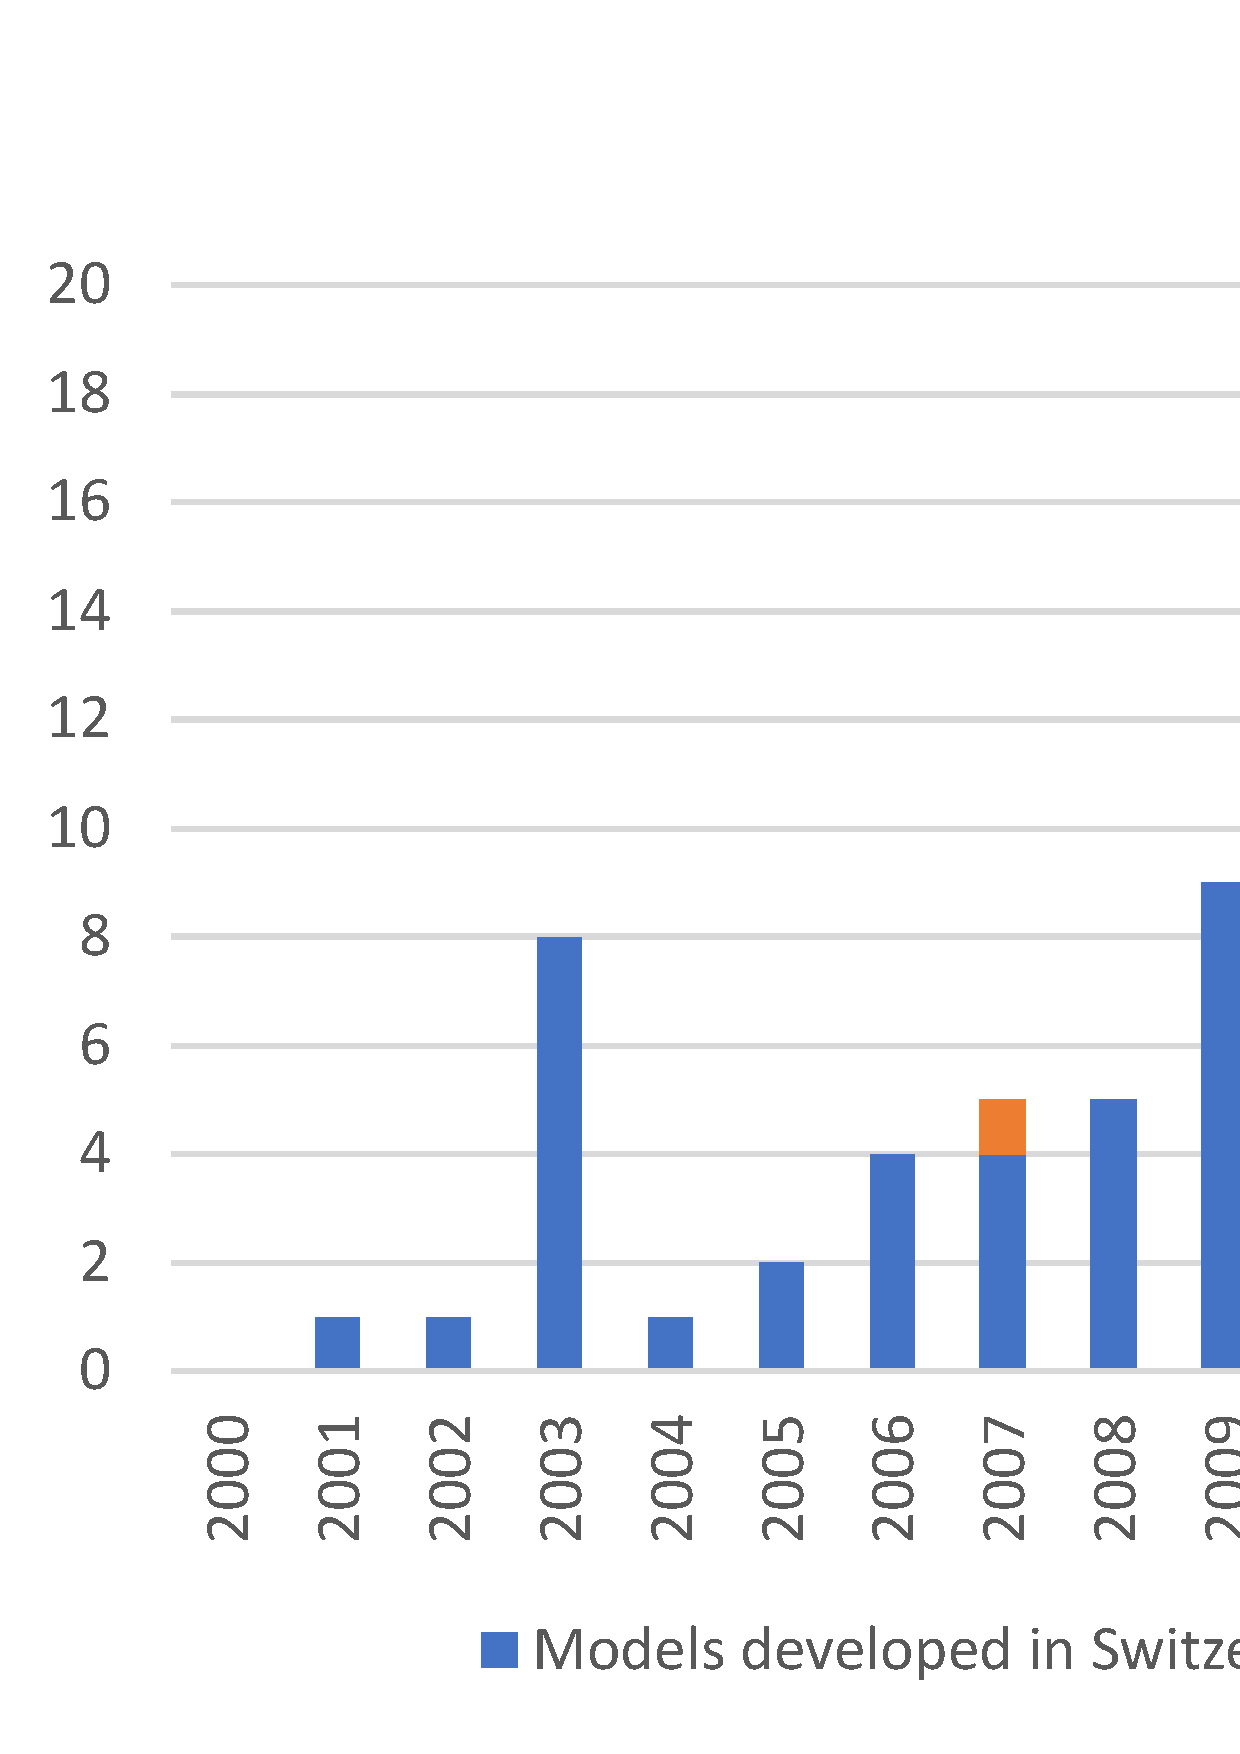
\includegraphics[width=0.70\columnwidth]{figures/histogram.png}
		\caption{{Number of articles reporting applications of hydrological models over the years with a distinction of the models developed in Switzerland and international models. {\label{fig:bars}}
		}}
	\end{center}
\end{figure}

\citet{Addor2019} argue that the choice of a model is driven by legacy rather than adequacy, where they understand by legacy: ``practicality, convenience, experience, and habit''. This hypothesis implies that the hydrological model of choice depends on the one hand essentially on the experience available in the modelling group and on the other hand on the code and data availability. Modeling habits also have positive aspects as they can contribute to efficiency and expertise \citep{Babel2019}.

In the articles analyzed here, about 25\% of the authors specifically address the model's adequacy with the context or the landscape. However, this does not mean that adequacy has been formally tested or that it actually drove the choice of the model, but rather that it is argued as suitable to the intended application. About 53\% of the articles do not provide any mention of adequacy. The rest provide some description of the model characteristics that might be interpreted as arguments for suitability to the case study. Furthermore, besides the hydrological processes studies (Section \ref{sec:application:process}), there are no examples where the perceptual model, i.e. the modellers' perception of how nature works, is explicitly discussed, a shortcoming that is the rule rather than the exception in hydrological modelling works \citep{Beven2021}.

\begin{figure}[htb]
	\begin{center}
		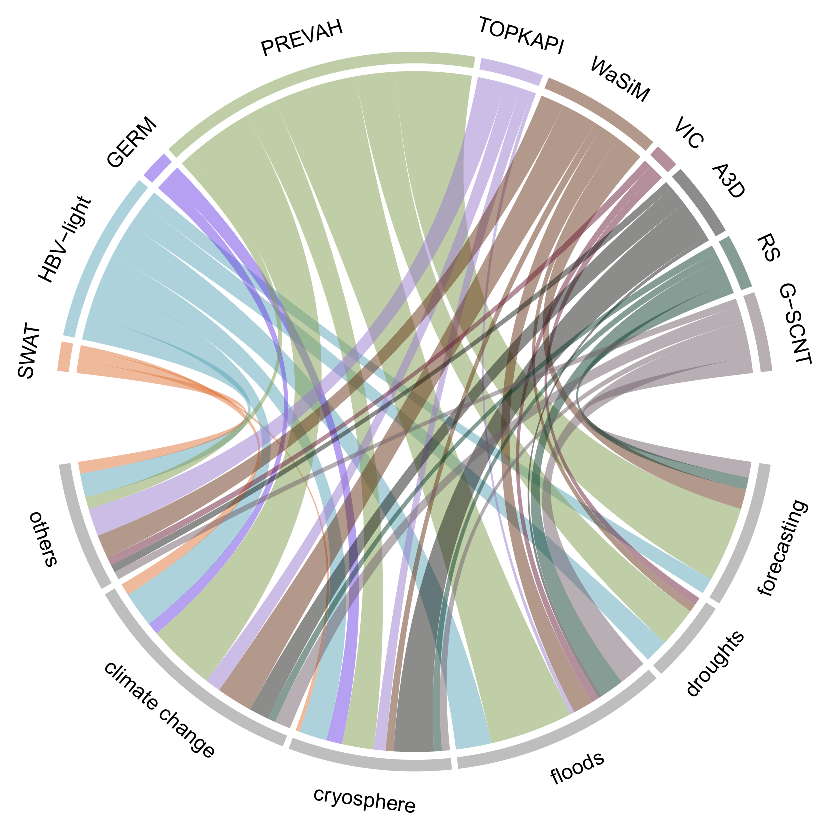
\includegraphics[width=0.70\columnwidth]{figures/chord_diagram_contexts}
		\caption{{Hydrological models applied to different contexts in Switzerland. The importance of the link is proportional to the number of scientific articles. The importance of some models can be inflated by the fact that an article can address multiple contexts, such as floods and climate change. Models with too few use cases (less than three) are not included for the sake of clarity. A3D stands for ALPINE3D and G-SCNT for GSM-SOCONT. 
		{\label{fig:applications}}
		}}
	\end{center}
\end{figure}

\begin{figure}[htb]
	\begin{center}
		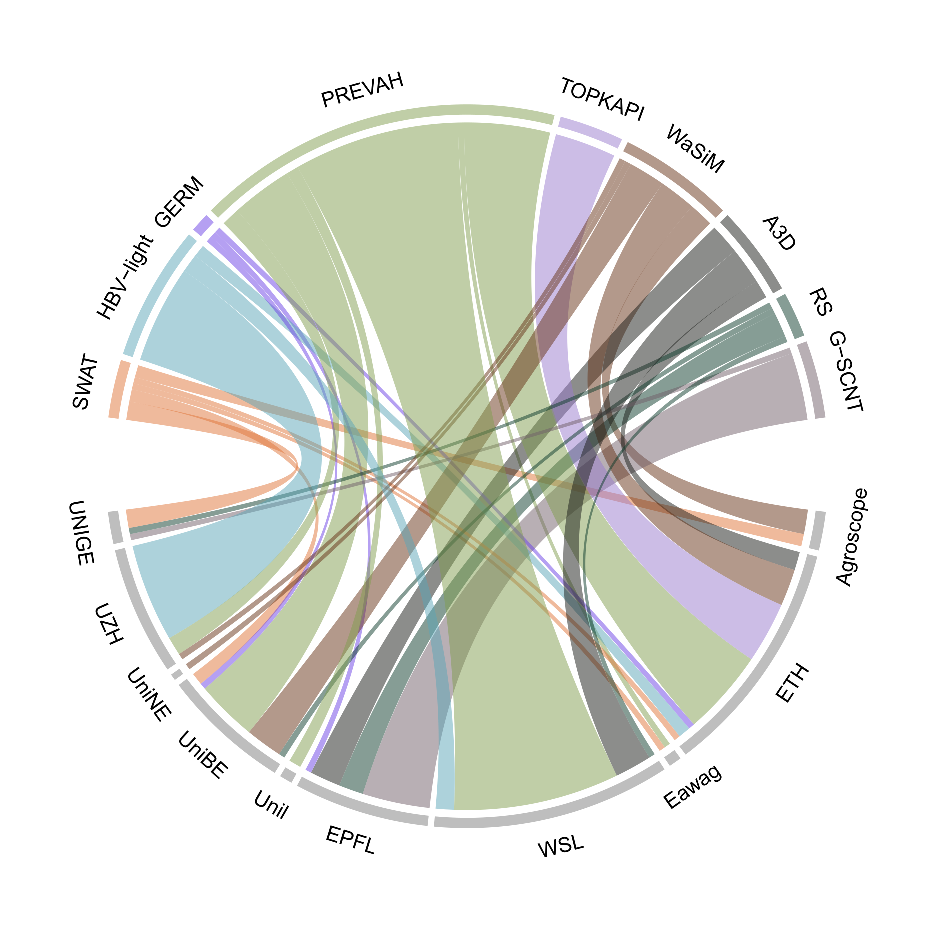
\includegraphics[width=0.70\columnwidth]{figures/chord_diagram_institutes}
		\caption{{Links between hydrological models and the Swiss institutes that use them. Same conventions as Fig. \ref{fig:applications}. Models or institutes with too few use cases are not included.
		{\label{fig:model_institutes}}
		}}
	\end{center}
\end{figure}

Some models are specialized for certain processes, such as ALPINE3D for snow and GERM for glaciers, and are thus proportionally more used in these contexts (Fig. \ref{fig:applications}). TOPKAPI-ETH tends to be more used for processes that need a physically-based representation or that need a gridded spatial structure to provide gridded output, e.g. in view of coupling to another model. RS specifically targets flood modelling and hydropower operations, as it was designed for operational flood mitigation with hydropower plants. The three most used models, i.e. PREVAH, HBV-light and WaSiM, are general models and are applied to different topics, such as climate change impact studies, floods, droughts, cryosphere-related processes, and operational forecasting (Fig. \ref{fig:applications}).

One point to note is that the adequacy to climate change studies is generally not discussed. References to previous studies are sometimes provided, without the latter having addressed this point explicitly. While it is relatively easy to demonstrate a model's ability to reproduce floods or drought conditions, its transferability to other climate conditions is more difficult to prove directly. 

One of the reasons driving the choice for one hydrological model, besides the adequacy, is reusing a model that is already set up for a catchment of interest, sometimes without the need to recalibrate it. About 20\% of the articles explicitly state that the applied model comes from another study. Likely, this number should be higher as some authors publish multiple articles targeting different topics but on one model setup, without explicitly mentioning it.

Another reason is the selection of the model that is developed and used at the research institute. This is a strong driver, as for 66\% of the articles the first author is affiliated with the institute where the model is being developed - which confirms a hypothesis that is indeed widespread in hydrology. The model at hand is thus well known, the code is available, and specialists are present to make necessary adaptations to it. Also, when the model is not one from the institute, collaborations are established with the developer or the lead researcher of the model, leading to the fact that for 72\% of the articles, the model developer (or team leader) is co-authoring the paper. These three aspects - reuse of an existing setup, in-house knowledge and collaborations - have one common ground, which is convenience. Finally, the choice of the model might also be imposed by a project.

While we see an impressive model diversity at the single or few catchments scale, it is noteworthy that our review points towards an important national-scale shortcoming: while there are catchments that have been ``over-modelled'' (e.g. Thur, Dischma) - however with little model intercomparison - there is a clear lack of large scale or national studies. In particular, the few available studies often do not cross the Swiss national border, even though the ``hydrological Switzerland'' extends to its neighbouring countries (Fig. \ref{fig:map}).

The absence of such larger scale studies might be explained by shortcomings and challenges more widely encountered in hydrological modelling over larger domains. These include differing quality and scales of input data and streamflow observations and large heterogeneity in hydrological behaviour (possibly requiring more than one specialized model). Yet, this heterogeneity may in fact provide us with the opportunity to improve our understanding of differences in model adequacy and model performance, and to draw most needed conclusions on the robustness of generalizations and on estimation uncertainty \citep{Gupta2014,McMillan2016}.


\section{On model structural uncertainty and multi-model approaches}
\label{sec:multi-model}


------------

Although there are currently few studies of this type, this topic holds potential for significant model diversification since hydrologic process analysis might require model structural changes to allow new hypotheses to be tested. An example is given by \citet{DalMolin2020}, who discusses, based on the SUPERFLEX framework, how to flexibly adapt the model structure to integrate new hypotheses about dominant hydrological processes.

The World Meteorological Organization (WMO) used to carry out comparisons of hydrological models and to publish the results in Operational hydrology reports. Different international models were compared over various catchments, including the Dischma basin in Switzerland. The Snowmelt Runoff Model \citep[SRM,][see supplementary material]{Martinec1975} has also been assessed in these early model comparisons \citep{WMO1986, WMO1992a}.

However, there are few model intercomparison studies in Switzerland, and none of them led to a preference of one model over the other, which is reflected in the fact that the recent re-evaluation of climate change impact on water resources involved all the major models developed in Switzerland  \citep{FOEN2021}. The existing model intercomparison studies are classical studies on what we can gain from model complexity in terms of model performance; e.g. \citet{Gurtz2003} compared PREVAH to WaSiM-ETH, \citet{Orth2015} HBV-light to PREVAH and a simple water balance model, \citet{Kobierska2013} ALPINE3D to PREVAH and \citet{Andrianaki2019} SWAT to ALPINE3D and PREVAH.

Very few studies use catchment-scale hydrological models to assist hydrological process research and hypothesis testing within a hydrologic model development framework \citep{Clark2016}. This might be explained by the fact that it remains highly challenging to draw conclusions on hydrological processes based on model simulations at the catchment scale; corresponding work rather involves small scale modelling at the hillslope scale (e.g. the study of \citealt{Heuvel2018} from the US).  

%Quantification of uncertainty sources in climate impact studies has been assessed by (Bosshard et al., 2013) for the Alpine Rhine using PREVAH and HBV. None of the assessed uncertainty sources was found negligible. The model’s impact was more important in winter and spring than in summer or autumn, where the climate models have a larger contribution. 

%There are only few model comparison studies in Switzerland. (Gurtz et al., 2003) compared PREVAH and WaSiM-ETH for two mountainous catchments, showing that both models perform with similar statistical efficiency. (Orth et al., 2015) compared HBV-light, PREVAH, and a simpler model for eight catchments, finding in like manner that added complexity does not necessarily lead to improved performance, and that this can vary greatly depending on the considered hydrological variable (e.g. runoff vs. soil moisture) or hydrological conditions (floods vs. droughts). (Kobierska et al., 2013) compared ALPINE3D to PREVAH (HRU version) for the assessment of future runoff from a mountain catchment with a glacier contribution. ALPINE3D was chosen as it is physically-based (for the atmospheric, snow and glacier modules), while PREVAH was selected as it is “particularly enhanced for applications in mountain regions”. (Andrianaki et al., 2019) assessed the performance of SWAT for the same glacierized catchment as (Kobierska et al., 2013). A different description of some underlying processes resulted in seasonal variability of model performance and in different findings, highlighting that results of climate change studies in glacierized basins can also strongly depend on the sensitivity of model’s parameters.

% (Addor et al., 2014) assessed the impact of climate change on hydrological regimes with the consideration of multiple sources of uncertainties, one of which was the choice of the hydrological model. They applied HBV-light, PREVAH, and WaSiM-ETH to six catchments in Switzerland and identified that the contribution of the hydrological models to the uncertainty was significant in (partially) glacierized catchments. This is in agreement  with (Kobierska et al., 2013), however here despite the different sources of uncertainty, a robust change in the hydrological regimes could be identified.

%(Dal Molin et al., 2020) for the development of a semi-distributed hydrological model using SUPERFLEX aiming at reproducing the dominant controls on streamflow spatial variability.

%(Melsen et al., 2019) analyzed the impact of modelling decisions on the model results, particularly for floods and droughts.

\section{Conclusion}
\label{sec:conclusion}

Focusing on Switzerland, we carried out a comprehensive literature review on the hydrological models developed and applied in different contexts. The objective of this work was to disentangle the motivations and reasons behind the choices that led to the current co-existence of a wide range of streamflow models in a small country. To structure the analysis, we attempted a classification into eight fields of model application, ranging from hydrological process research to model uncertainty analysis and large scale modelling. For all reviewed studies, we examined the arguments that were explicitly put forward by the authors for model selection, as well as implicit aspects, such as the author's affiliation or co-authorships. 

The model adequacy for the study context or the landscape is explicitly addressed by only 25\% of the articles, while 53\% make no mention of adequacy, neither provide any justification for the choice of the model. The models that have specifically been developed to represent specific processes, such as snow- or glacier melt or hydropower operations, are obviously mainly used in these contexts. However, the more general models, which are also the most used ones, are applied indifferently to various contexts and landscapes.

Not surprisingly, researchers active in Switzerland are very keen on using a model developed in Switzerland (93\% of the case studies) or even at their own research institute (66\% of the articles analysed), and possibly used on the same catchment previously (20\%), which all in all underlines that convenience might be the foremost model selection driver. Moreover, this is likely to be the cause of the existence of so many hydrological models, as each research group develops its own tools.

Convenience certainly also explains that some catchments are used in numerous studies and that larger scale or multi-catchment studies on hydrological functioning and model behaviour are largely missing: both points might in fact be explained by how tedious it remains to gather all relevant data (Switzerland does not yet have a hydrological data portal). The absence of model intercomparison, in exchange, might at least partly be explained by the few open-source models used in
Switzerland. 

With ongoing climate change and ensuing challenges for water resources and water-related hazard management, hydrological modelling needs to evolve quickly. In Alpine environments, the most striking example is certainly the emergence of hydrological droughts \citep{VanLoon2015} during summer and fall \citep{Brunner2019e, Rigling2020}, which requires to understand the drivers of low flow \citep{Arnoux2020} and the development of hydrological models that reliably represent groundwater recharge.

This component is, in fact, crudely parametrised in many streamflow models for alpine environments. Improved modelling of surface water-groundwater interactions is also a pre-condition for water temperature projections, agricultural water use and related water quality, drinking water management, and biodiversity assessment in ecosystems strongly influenced by river-groundwater interactions \citep{Brunner2017}. 

Another key topic that will receive growing attention is the role of the vegetation in modulating climate extremes \citep{Mastrotheodoros2020} and land-use changes induced by climate warming, calling thereby for improved representations of vegetation's role in hydrological models.

Accordingly, application-oriented as well as essentially research-oriented models can see further diversification in the near future. If model development continues the path taken so far, models will branch into sub-variants, and process-specific models will be created. However, we see two elements that might reverse the trend. The first element is the emergence of modular frameworks that allow creating a wide variety of model structures. While some specific topics might still need custom models tailored to certain applications, most hydrological models share similar principles and process representations. The creation of such flexible frameworks is strongly encouraged by \citet{Clark2011a}. Nowadays, different flexible frameworks exist, such as SUPERFLEX, FUSE \citep{Clark2008}, PERSiST \citep{Futter2014}, ECHSE \citep{Kneis2015}, MARRMoT \citep{Knoben2019}, Raven \citep{Craig2020}, and SUMMA \citep{Clark2015}. {However, the flexibility provided by these frameworks likely comes with a counterpart, which is more code complexity. Most of these frameworks are relatively new and their adoption by a large community of modellers remains to be proven}.

The second element is the growing adoption of version control systems that allow collaboration on open-source code with unprecedented ease. These code sharing platforms (code repositories) allow for anyone to suggest improvements (in a written form) to an open-source code or even to suggest changes to the code (e.g. pull requests) that will be reviewed by the developers of the model and merged to the main code base. As more models go open source, the need to create in-house versions to implement processes decreases. Hopefully, it should increase contributions to shared code bases and benefit a community-driven dynamic that would be beneficial for all, increasing thereby international collaborations.


\section*{Acknowledgements}

We would like to thank various colleagues for their help on the history of hydrological modelling in Switzerland (see Supplementary Information) and Karsten Jasper for the insight on hydrological modelling at the Swiss Federal Office for the Environment (FOEN).


\section*{Appendix 1: Short model descriptions, alphabetical order}
\label{appendix:1}

\textbf{ALPINE3D} \citep{Lehning2006} is a model developed in Switzerland targeting surface processes in alpine environments, in particular snow processes, and is suitable for very steep terrain. It targets applications where the small-scale variability at the atmosphere-surface interface is important. Three-dimensional aspects relate to processes in the atmosphere, such as drifting snow. The snow-related processes are modelled by the physically-based SNOWPACK model (\citealt{Bartelt2002, Lehning2002a, Lehning2002b}). ALPINE3D has a built-in runoff module adapted from an early version of PREVAH \citep{Lehning2006} and a runoff module that solves the Richards equations \citep{Wever2017}. It has been recently extended by a hydrological simulation tool for streamflow and water temperature prediction \citep{Gallice2016}.

\textbf{CemaNeige-GR6J} is the daily version of a lumped, bucket-type rainfall-runoff model with six free parameters \citep{Pushpalatha2011}, combined with the CemaNeige snow module \citep{Valery2014a, Valery2014b}, which is a routine for snow accumulation and melt based on a degree-day concept that introduces two additional free parameters. GR6J is an empirical model with a root zone storage and two routing routines: one for the slow (unit hydrograph) and one for the fast flow component ({unit hydrograph}, a non-linear and an exponential store). Both flow components interact with the groundwater through an exchange coefficient. It has seen one application in Switzerland for a climate change impact study \citep{Keller2019a}.

\textbf{DECIPHeR} (Dynamic fluxEs and ConnectIvity for Predictions of HydRology; \citealp{Coxon2019}) is an open-source flexible model framework suited for different spatial scales. The model builds on the code and key concepts of Dynamic TOPMODEL (\citealp{Beven2001}), an improvement of the original TOPMODEL (TOPography based hydrological model; \citealp{Beven1979}). It can be run as a lumped model (1 HRU), as semi-distributed (multiple HRUs) or as fully distributed (HRU for every single grid cell). Each HRU is treated as a separate functional unit in the model and thus allows for different process conceptualizations and parameterizations across the catchment.

\textbf{GERM} (Glacier Evolution Runoff Model; \citealt{Huss2016, Farinotti2012}) consists of five different modules, which largely rely on existing approaches, dealing with snow accumulation, ablation, glacier evolution, evapotranspiration and runoff routing. It is a fully distributed, deterministic, conceptual model designed mainly for simulations at a daily resolution and a high spatial resolution. Glacier geometry is updated annually according to a non-parametric approach proposed by \citet{Huss2010}. The hydrological module is based on the concept of linear reservoirs and distinguishes five surface types: ice, snow, rock, vegetation and open water. 

\textbf{GSM-SOCONT} (Glacier and SnowMelt -- SOil CONTribution model; \citealp{Schaefli2005c}) is a semi-lumped conceptual glacio-hydrological model composed of the reservoir-based SOCONT model (consisting in a linear reservoir for the slow soil contribution and a non-linear reservoir for direct runoff) and the GSM model for the glacierized area. the SOCONT model was inspired by the GR3 model \citep{Edijatno1989}, which is part of the GR model family as is CemaNeige-GR6J (see above). It was developed at the Ecole Polytechnique Fédérale de Lausanne (EPFL). The model has a parsimonious structure and was initially developed for climate change impact studies. Catchments are subdivided first into ice-covered and ice-free parts and then in elevation bands. A version of GSM-SOCONT has been implemented into RS (see below) and modified for operational flood forecasting \citep{Hamdi2005} and for design flood estimation \citep{Zeimetz2018}.

 \textbf{HBV} (Hydrologiska Byråns Vattenbalansavdelning model; \citealp{Bergstrom1976a, Bergstrom1992, Bergstrom1995, Lindstrm1997})  is a rainfall-runoff model that focuses on runoff generation processes, including snowm, and is characterized, by its original developers \citep{Bergstrom1992}, as being very general and is thus applied in many different geographical and climatological conditions. 

\textbf{HBV-light} \citep{Seibert2012} is an implementation of the HBV model (see above) that is further developed at the University of Zurich. HBV-light corresponds to a simplified and userfriendly version of the original model. 

\textbf{HYPE} (HYdrological Predictions for the Environment, \citealp{Lindstrom2010}) is a large-scale semi-distributed conceptual model, designed to simulate discharge and model flow paths of nutrients in the water, and was originally developed by the Swedish Meteorological and Hydrological Institute. In the model, the landscape is divided into classes according to the soil type, land use and altitude, and the parameters are either global or coupled to the soil type or land-use. The model can simulate natural hydrological processes of snow- and glacier melt, evapotranspiration, soil moisture, groundwater and routing through rivers and lakes, but also human-induced influences, such as regulated lakes and reservoirs, water abstractions and irrigation. HYPE is run operationally by SMHI for several purposes (e.g. flood forecasting or climate change impact assessments). The version covering the pan-European continent is referred to as E-HYPE, its application is entirely based on open and readily available data sources \citep{Donnelly2015}, including historical data (1981-2010), 1-10 day forecast, seasonal forecasts, climate change impact scenarios and actual model performance (\url{https://hypeweb.smhi.se/explore-water/geographical-domains/\#europehype}).

\textbf{LARSIM} (Large Area Runoff Simulation Model; \citealp{Ludwig2006}) is a semi-distributed hydrological model, which describes continuous runoff processes in catchments and river networks. The model structure (subunit) can be grid-based or based on hydrologic subcatchments. While runoff generation (described with parallel linear storage reservoirs), routing (depending on channel geometries and roughness conditions) and flow retention are simulated at the subunit scale, snow storage, evapotranspiration, interception and soil storage are simulated at a subscale level according to land use classes. While it doesn't include a glacier melt component, LARSIM includes many features that were specifically designed for its operational use as a flood forecasting model, as well as offline applications \citep{Stahl2017}. 

\textbf{LISFLOOD} is a GIS-based model for catchment-scale water balance simulation \citep{vanDerKniff2010}. It has been specifically designed for large river catchments, and in particular, it makes use of data layers that are available for the Joint Research Center (JRC) at European scale, such as land use, soil type and texture, river network \citep{Thielen2009}. LISFLOOD is used by the European Flood Awareness System, EFAS, for medium- and seasonal-range forecasts with a 6-hourly and daily time step. Both historical river discharge time series (1991 to near real-time) and reforecasts (1999-2018) are available on the Climate Data Store of Copernicus (\url{https://cds.climate.copernicus.eu/}). 

\textbf{mHM} (mesoscale Hydrological model; \citealt{Samaniego2010a, Kumar2013, Thober2019}) is a distributed hydrological model, which has the particularity of using the multiscale parameter regionalization approach (MPR, \citealp{Samaniego2010a}) for parameter identification. It has been specifically developed to not need recalibration when applied at different resolutions \citep{Kauffeldt2016}. It is driven by hourly or daily meteorological forcings and utilizes observable basin physical characteristics to infer the spatial variability of the required parameters. It is developed by the Umweltforschungszentrum Leipzig and has been successfully applied to catchments ranging from 4 km\textsuperscript{2} and to beyond 500,000 km\textsuperscript{2}. To the best of our knowledge, it does not yet have a glacier melt component. The open-source code (Fortran) is available at \url{https://git.ufz.de}.

\textbf{PREVAH} (Precipitation-Runoff-Evapotranspiration HRU Model; \citealt{Gurtz1999, Viviroli2009a}) is a Swiss conceptual model that has been developed specifically for heterogeneous mountainous environments with highly spatially and temporally variable processes. It follows the HBV model structure, with numerous modifications, and was designed for studies in Alpine headwater basins \citep{Orth2015}. PREVAH branched out into different versions, two of which are mostly used: an HRU-based version that runs at an hourly time step and a fully distributed version \citep{Zappa2012} that runs at a daily time step. The distributed version of PREVAH being the most used, any reference to PREVAH in this paper implies the distributed version if not stated otherwise.

\textbf{RS} (Routing System; \citealp{Dubois2000, GarciaHernandez2020, Foehn2020}) has been developed at the Swiss Federal Institute of Technology in Lausanne (EPFL). The version that is freely available, and thus more used, is RS MINERVE, which was developed for operational flood forecasting in Valais \citep{GarciaHernandez2009b} and which is maintained by the CREALP (Centre de recherche sur l'environnement alpin). RS specifically targets hydropower systems by modelling the influence of regulated infrastructures and thus allows modelling complex hydrological and hydraulic networks with anthropogenic influences.

\textbf{SEHR-ECHO} (Spatially Explicit Hydrologic Response model for ecohydrologic applications; \citealp{Schaefli2014}) is an evolution of GSM-SOCONT that was developed at the Swiss Federal Institute of Technology in Lausanne (EPFL). The model aims at taking into account the spatial variability in the runoff generation. The catchment is divided into subcatchments connected to the river network in order to account for the origin of the different areal contributions and to route them in the river network. 

\textbf{StreamFlow} is an extension of ALPINE3D (see above). It uses an explicit formulation of travel times \citep{Comola2015}, as does SEHR-ECHO (see above). 

\textbf{SUPERFLEX} \citep{Fenicia2011a, Kavetski2011} is a flexible hydrological framework now developed at Eawag (the Swiss Federal Institute of Aquatic Science and Technology). It allows building hydrological models using generic components for hypothesis testing. The building blocks are reservoirs, lag functions, and connections. The models elaborated with SUPERFLEX can be lumped, semi-distributed \citep{Fenicia2016} or fully distributed \citep{Hostache2020}. An open-source version written in Python is available \citep{DalMolin2020a}.

\textbf{SWAT} (Soil Water and Assessment Tool; \citealp{Arnold1998}) is an open-source semi-distributed, process-based hydrological model. Besides hydrology, other SWAT components can simulate energy balance, soil temperature, mass transport and land management at the sub-basin and HRU levels. It is one of the most applied models worldwide probably because of the broad range of hydrologic and environmental problems that can be addressed with it.

\textbf{TOPKAPI-ETH} \citep{Finger2011, Ragettli2012}, developed at ETH Zurich, is a branch of the TOPKAPI model (TOPographic Kinematic APproximation and Integration; \citealp{Todini1995, Todini2002, Liu2002, Ciarapica2002}).  It is a fully distributed and physically-based model based on the spatial integration  of the kinematic wave model over the pixels of the digital elevation model (DEM). TOPKAPI-ETH has been modified for application to mountain basins by adding a second soil layer and modules for snow, glaciers, reservoirs, water abstraction, and diversion, and a new evapotranspiration scheme \citep{Finger2011, Finger2012, Fatichi2015}. 

\textbf{VIC} (Variable Infiltration Capacity model; \citealp{Liang1994a}) is an open-source grid-based land surface hydrological model. It is implemented so that grid cells with a resolution up to 1km are simulated independently of each other. Sub-grid heterogeneity introduced by different land-use types and elevation is handled via statistical distributions. Routing must be performed separately with an additional routine taking care of the water transport between cells.

\textbf{WaSiM} (Water Flow and Balance Simulation Model; \citealp{Schulla2007, Schulla2009}) is a fully distributed hydrological model originally developed at ETH Zurich under the name WaSiM-ETH. It describes the water fluxes in the unsaturated soil using the 1D-Richards equation \citep{Richards1931}. The transfer function (runoff concentration) can be processed through a series of linear reservoirs or with the kinematic wave approach (from one cell to another). WaSiM covers a wide range of hydrological processes relevant for alpine environments, with different implemented variants.

\textbf{wflow} is the modular and distributed hydrological modelling platform of DELTARES (\url{https://www.deltares.nl/en/software/wflow-hydrology/}). \textit{wflow\_hbv} is a fully distributed version of the conceptual HBV model \citep{Lindstrm1997} - applied on a grid basis - in the wflow framework with a kinematic wave as routing instead of the original triangular routing function; the model has an interception reservoir, snow module, root zone storage, fast runoff reservoir, and a groundwater reservoir \citep{deBoerEuser2017}. 


%\FloatBarrier
\bibliographystyle{ametsoc2014}
\bibliography{biblio}

\end{document}

